\documentclass[11pt]{article}
\usepackage{times}
\usepackage{amsfonts}
\usepackage{color}
\usepackage{multirow}
%\usepackage{rotating}
\usepackage{url}
\usepackage{latexsym}
\pagenumbering{arabic}
\usepackage{graphicx}
\title{Location-Based Dynamic Social Networks}


\author{
   Vladimir Eidelman, Raul Guerra, and Jim Stevens\\
Department of Computer Science \\
University of Maryland, College Park\\
   %\affaddr{College Park, MD 20742}\\
 { \tt \{vlad,rguerra,jims\}@cs.umd.edu}
}
\begin{document}

\maketitle 

\section{Introduction}


Technology, especially internet-based technology, has often been portrayed as having an alienating force by further removing us from `real' social interaction in favor of the virtual kind. However, a wave of recent applications has shown that in fact, the opposite can be true. Services such as Foursquare, Hot Potato, and Meetup have shown that we can actually enhance `real' experiences through the use of technology. 

In this paper, we present our efforts to extend that line of thinking in the form of location-based dynamic social networks. Imagine walking into a classroom or party, and having access to a dynamic social network with the other people in your immediate area, including desired profile information and real time information which is dependent on the venue. Motivated by the previous idea, the Proteus group implemented an application that generates dynamic networks that are location dependent for a user to immediately recognize people of interest or for a user to establish contact more easily with other users. The main objective is to facilitate interaction with new people around you who may potentially match your interests. The secondary objective is to find out if your friends are around and get together. 

The rest of this paper is structured as follows. First, we will present our overall system architecture in Section 2, including backend logic, database interaction, and user interfaces. Then, we will outline the implemented use cases in Section 3, followed by a discussion of future extensions in Section 4.


\section{System Architecture}

\subsection{Overview}

For the user, all interaction with the application takes place through a web interface. The first interaction users have is creating an account on the system. At this point, the user provides their profile information. This will also be used by the recommendation engine to match other users of interest. A user's profile resembles an online business card, only containing information they are willing to share with other people, since the emphasis is not in sharing personal information, but rather on encouraging real interaction. 

To complement the profile information, the user is constantly updating his or her context information. This includes active updates, where the user himself provides additional status information, like a list of interests, and passive updates, like location, where the users information is updated by the application automatically. The context information, in addition to the profile, is used by the application to find other users of interest. 

The interface interacts with a server to find other nearby users and, along with their context, displays the network of users logged in at a specific location in a Google Maps interface. Through the Google Map interface, the user can see other users' real time location, their profile information, links to other social media, such as Facebook and Twitter, and have an option to interact with them. 


As our application is web-based, it can run on any computer or mobile device which has a web browser, making it extremely portable. Making it light-weight in order not to unduly drain the limited resources of a mobile device was also a design priority, and thus all computation is performed on the servers, and only the necessary map update process runs on the device itself. 

However the application does need device specific information, the GPS location of the device running the application. This is not a problem because as the HTML5 standard becomes more pervasive, this application will be able to be deployed in any cellphone, PDA, iphones, etc. whose browser supports HTML5 geolocation capability.

%%diagram
Figure ~\ref{fig:arch} shows the structure of our system, as currently implemented. 
 
\begin{figure}[h]
\begin{center}
  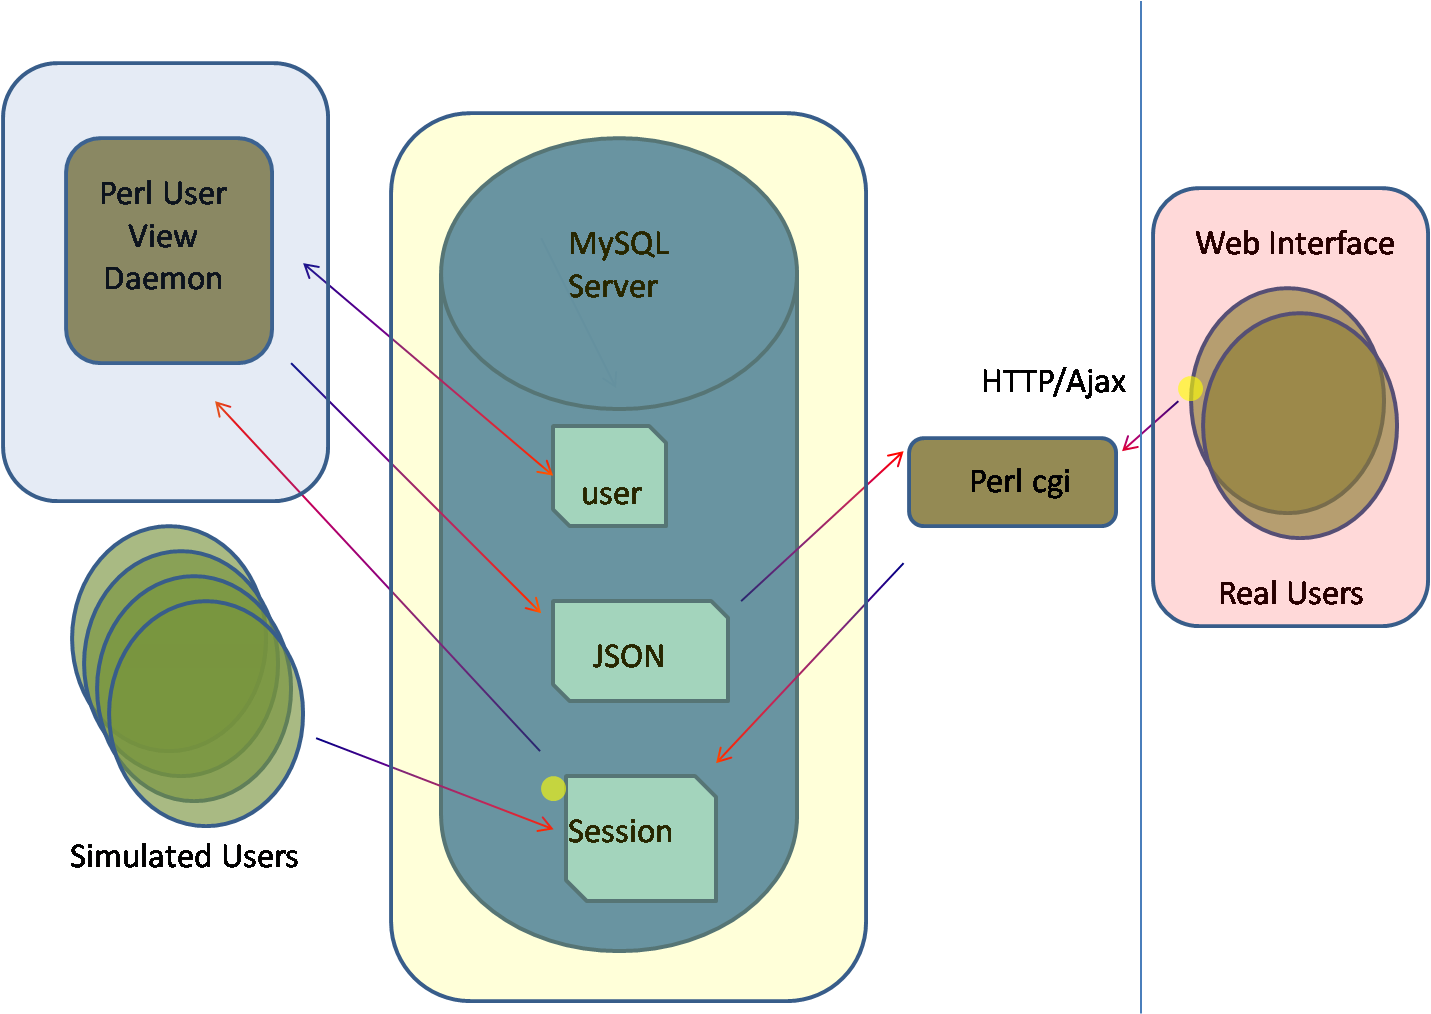
\includegraphics[scale=0.5]{sysarch.png}
\caption{System architecture}
\label{fig:arch} 
\end{center}
\end{figure}



\subsection{Database Setup}

%%database names and descriptions

While using the application, users will enter and leave the dynamic social network continuously, depending on whether a person is considered to be `present' in the network or not. To determine whether a person is considered to be `present', the application will use GPS information from the user's browser. 

\subsection{User Interaction}

%%user interface
Figure ~\ref{fig:phoneapp} shows the proposed interface for a mobile device.
 
\begin{figure}[h]
\begin{center}
  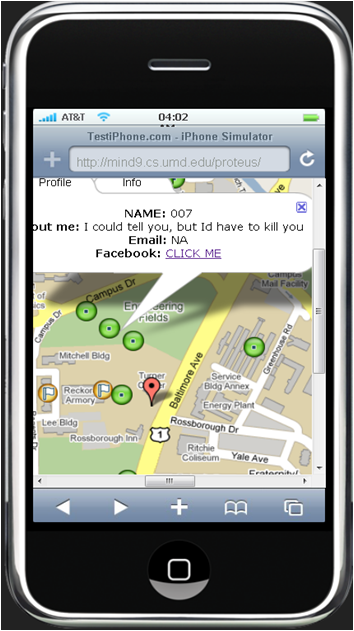
\includegraphics[scale=0.5]{phoneapp.png}
\caption{Example Apple iphone interface}
\label{fig:phoneapp} 
\end{center}
\end{figure}


The Google Map interface interacts with the backend both actively and passively. Actively, whenever a user wishes to query for other users in close proximity to himself or post a Graffiti tag. To do this, the user submits his request to a CGI script written in Perl, which parses the query and performs the appropriate action {\color{red}  queries the database} . Passively, while a user is logged into the system, the interface sends timed continuous updates indicating that the user is still active, and providing an updated location in the form of (longtitude, latitude), indicating the user should remain in the session table. {\color{red}  Indicate what a session table is and how it relates to the CGI script or don't mention it} In both cases, the script takes the information and inserts it into the appropriate places in the database. 

Then, the script asynchronously polls the JSON table {\color{red}  JSON table where? Need to explain what the JSON table is and where does it fit in all of this or remove it} , providing the map interface with the updated position, status, timestamp, etc. of the users which are in close proximity. 

\subsection{User Interface}

We currently support two different user interfaces, which we subsequently describe as location-based and name-based. The two views compliment each other in that the location view is useful for presenting a user with the layout of surrounding users, to encourage interaction with new people in the immediately surrounding area, and the name view facilitates interacting with already known users. also the name view is perfect for quickly browsing Graffiti tags, as opposed to finding all of the Graffiti tags in the map and clicking one by one to find one of interest. Figure ~\ref{fig:map1} presents the location view, which is the Google map interface that the user encounters upon logging into the system. In this interface Flags represent Graffiti tags and Green dots represent users.

Figure ~\ref{fig:userlist} presents a complimentary interface which allows users to scroll through a list of usernames to locate known friends.

\subsubsection{Google Mashup}

To implement the location view interface our web application makes extensive use of Google Maps and its API \url{http://code.google.com/apis/maps/documentation/reference.html}.  The API makes it easy to display a Google Map, Graffiti tags, and users, the last two are just Google Map markers with different icons.

Not only does the web application send information to the server, as mentioned earlier, it also gets information continuously from the server. At the same time the web application sends information it receives information. Thus the web application receives timed continuous updates with the most up-to-date location of all the logged-in users. 

The web application keeps track of the users that it is currently displaying, because there are two types of updates it performs. First, if the web application receives a new user from the  backend server then it updates the Map with a new marker. If it receives an update for a users it is already displaying then the web application updates the latitude and longitude of the marker in the map. Having these two type of updates, as opposed to creating all the users each time it receives an update,  makes the movement of the users in the map much smoother. However, this increases the overhead of the web application. As mentioned above a user through the web application send continuous updates to indicate the he or she is still active. Thus an inactive user is one that is not continuously updating its location. These type of users are no longer present in the social network or inactive. When this happens the backend server stops sending information about a user and the web application stops displaying him or her in both the Map and the names list.

Both interfaces share a lot of the functionality. When a user is added to the Map, this user is also added to the list of users in the name-based interface and the same when a user is removed.

An interesting part of the user interface that is not necessarily part of the location-based or name-based interfaces is the play/pause button. The purpose of this button is to stop both interfaces from updating until the button is pressed again. This facilitates the interaction of one user with the rest of the users. WIthout the button a user would have to chase a user as it moves through the map to be able to click on it and see that user's profile. On the other hand, by clicking the button a user can freeze this virtual world and easily click on whatever user he or she wants.


\subsubsection{Graffiti/Tagging}

The Graffiti capability sprung from the concept of social tagging and the idea of personalizing a place for the duration of the dynamic social network. This functionality allows users to actively comment on the particular venue and passively input information into the web application system that could be used for a variety of purposes. One is that the recommendation engine could use this input and match users whose Graffiti behavior is similar. Another is using the Graffiti information to try to predict a user's behavior. For example, if a user has posted negative Graffiti in a restaurant, the web application can take this into account next time it recommends a place to eat. The final example is that Graffiti can be used as an indirect way of communicating. The Graffiti can be a forum where lots of users post messages. However, Graffiti differs from forums because it is transient and it only exists for the duration of dynamic social network. Thus, Graffiti more closely resembles a group of people gathering at a place to gossip than a forum.

Currently Graffiti is the only way for users to communicate through the web application. As mentioned before to do this a user leaves messages at specific locations and other users can see these messages and leave their own.

\subsubsection{Business Card/Profile}
For the purpose of building the framework of the web application and having the least amount of constraints while building it, we assumed that all the logged-in users trust each other.  Because of this, there is no point in having anonymous users and each user should have a profile with his or her information on it and be able to share it with others. Because the purpose of the web application is not to keep a repository of information for each user like Facebook, and our application seeks to facilitate social interaction among users, the profiles are slim and provide just enough information for a user to decide whether to interact with another or not. Hence the Business Card/Profile.

\subsection{Modularity}

%%how we can plug in/out fake users


\subsection{Daemon}


\section{Simulation}


In order to both validate the concept of our system and assess the structural limitations, we were inclined to design a simulation wherein we created virtual users. Utilizing the modularity described above, we were able to create an additional program which generated virtual users and updated their location, as if they were walking around campus, and plug it into our existing system as if the upates were coming in from real users. 

The program generates 25 virtual users in random locations within College Park, along with their profile information, which includes emails and Facebook links. Then the program assigns one of 16 possible destinations for each user, and moves each user at a random reasonable rate toward their chosen destination, updating the appropriate tables in the database at the normal time intervals. The list of possible destinations includes itesm such as AV Williams, Stamp Student Union, the library, and downtown. Once a user reaches the assigned destination, a new one is chosen for them at random and the simulation proceeds. 

While the simulation is active, a real user can log into the system and interact with any one of the virtual users. Using the simulation provided us with a convenient way of presenting our vision for what the real application interface would feel like, as depicted in Figure~\ref{fig:sim1}. 


\begin{figure}[h]
\begin{center}
  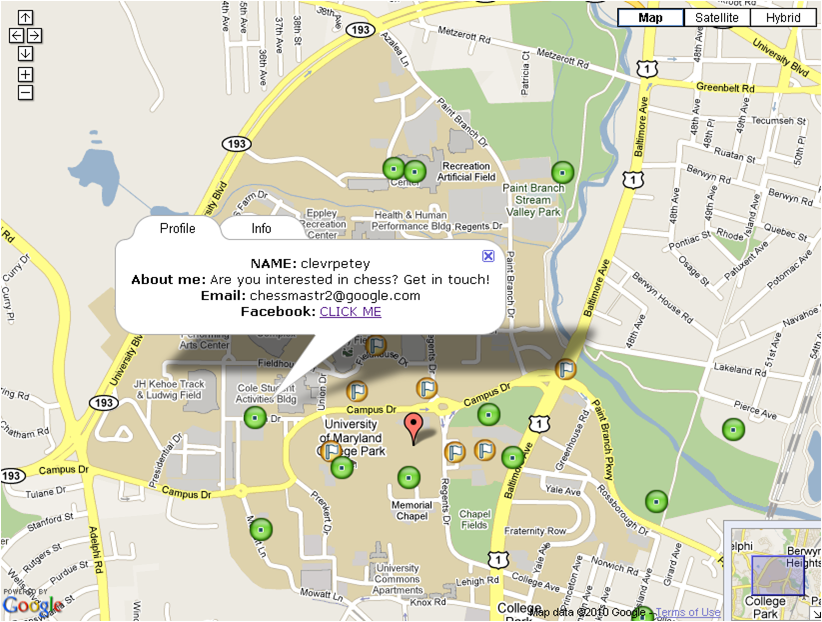
\includegraphics[scale=0.5]{sim1.png}
\caption{Example Apple iphone interface}
\label{fig:sim1} 
\end{center}
\end{figure}



\section{Future Work}
\subsection{Extensibility}

The project's biggest value resides both in the services it provides and the services it can be extended to provide, and the data it will produce once it is deployed. The application will produce a new type of social network data. While using the application, the users will be part of a complex social network which will be created and destroyed ad hoc in a short period of time. This will ellicit social interactions that do not happen in more rigid social networks like Facebook. This new type of data will raise questions in the area of Information Visualization, how can this rapidly changing data be best presented to a user? Machine Learning, how can this rapidly changing data be used by a learning system to infer information about the user? 

 If the application becomes as widely used as other Social Networks, then more structural questions are raised. What other hardware should be added to a mobile device to extend the application's capabilities or to make the information handling faster? Networks, would other design structures (like peer-to-peer) improve the performance of the application?

By no means is the application limited only to facilitating social interactions. The application's capabilities can be extended to provide almost any service that is location dependent. 


Furthermore the application's services can be complemented by any information captured by sensors currently in and in future mobile devices by capturing the context around the user. This data can be used to better inform the server about a user's surroundings and for the server to make better inferences about the user's surroundings and make suggestions to the user. For instance, we see a strong potential for collaboration with the TagMeAr groups virtual reality application and our social network, in visualzing the network and providing additional services.

Currently the framework for this new type of social network application is done. Users can create an account with their profile information, and they provide their real time location as their context. The Google Maps interface does show all the logged in users at a specific location moving in real time and allows a user to see other users' profile information and interact with them by clicking on their icon and getting their profile information.

Another capability we forsee in the future is the capability of users interacting directly with each other either through a chat client or a web cam.

Improve the way the server recommends users
Another future capability is the import of data from interactions previously made in the application. For example, a user can keep track of who he or she talked to during an event, and after the event he or she can choose to keep a link through exporting it to a more permanent social networking. Then, using profile information and algorithms yet to be developed, we can decide how best to present the other members of the current dynamic networks to the user, so that they can see that they do know someone at the party, or that their friend is right next door having lunch.

{\color{red} 
{\it PARAPHRASED THIS PARAGRAPH IN A FEW SENTENCES A FEW PARAGRAPHS UP I dont think we should put it in this way, sounds to negative, like we didn't do anything, but I haven't modified it yet}
Currently the application only implements very general and simplified versions of the services previously described. In the current application, users can create an account with their profile information, and the only context information they provide is their real time location. Because of the limited context information, the user recommendation engine could not be implemented; there is not enough information to recommend one user over another. The Google Maps interface does show all the logged in users at a specific location moving in real time and allows a user to see other users' profile information and interact with them by writing in other users' walls. Future work would focus on the back end; implementing a recommendation engine;  making the application deployable; and making the application scalable.
}


 \section{Conclusion}
 
 Our system is not unique, similar systems have been made, as mentioned earlier, to enhance 'real'' experiences through the use of technology. However unlike these other systems the web application described in this paper is trying to enhance 'real' experiences in a localized and personalized way. The main focus of the application is not to allow a user to reach out to millions of other users. Instead, the web application seeks to improve the user interactions with his or her acquaintances and to create connections that were not previously there between users.   
 
Our web application gives a new perspective to Heraclitus (c. 500 B.C.) famous saying "One can't step into the same river twice, since the river never remains the same" by updating it to "One cannot visit the same dynamic social network twice, since a social dynamic network never remains the same users constantly enter and leave".



\end{document}



